\documentclass[11pt]{article}
\usepackage[letterpaper,margin=.25in]{geometry}
\usepackage{amsmath,amssymb,booktabs,array,tabularx,xcolor,tikz,hyperref,embedfile,microtype}
\usetikzlibrary{trees}
\hypersetup{colorlinks=true,urlcolor=blue!55!black}
\pagestyle{empty}
\setlength{\parindent}{0pt}
\setlength{\parskip}{4pt}
\linespread{1.035}\selectfont
\definecolor{navy}{RGB}{25,54,86}
\definecolor{soft}{RGB}{244,247,250}
\tikzset{branch/.style={circle,draw=navy,line width=.6pt,inner sep=2pt},trueleaf/.style={circle,draw=navy,fill=navy,inner sep=2.1pt},falseleaf/.style={circle,draw=navy,fill=white,inner sep=1.8pt}}
\newcommand{\sectionbar}[1]{\vspace{3pt}{\color{navy}\bfseries #1}\par\vspace{2pt}\hrule\vspace{4pt}}
\begin{document}
\enlargethispage{.12in}

\embedfile[desc={A120603 exact certificate payload},mimetype=application/json]{certificate_payload.json}
{\color{navy}\LARGE\bfseries A120603 concise calculus certificate}\hfill{\small VERIFIED}\\[-1pt]
{\small Bradley Klee, \quad Mech.An.ika Sol (Open AI) \hfill July 31, 2026}

\sectionbar{Definition and first terms}
\(\displaystyle 16\,A(x)=15+27\,x+A(x)^{7}\), with the origin-normalized solution.\\
{\footnotesize Normalization/grammar: \texttt{A(x)=1+(3)*T(x); T=x+7*T\textasciicircum{}2+35*T\textasciicircum{}3+105*T\textasciicircum{}4+189*T\textasciicircum{}5+189*T\textasciicircum{}6+81*T\textasciicircum{}7}.}\\
\(a(0),\ldots,a(7)=1,3,21,399,9135,233709,6400947,183585897\).\\[2pt]
{\small Kernel used throughout: \(\displaystyle \rho(u)=u\,(1-7\,u^{1}-35\,u^{2}-105\,u^{3}-189\,u^{4}-189\,u^{5}-81\,u^{6})\), so \(x=\rho(T(x))\).}

\sectionbar{Typogeometry}
\begin{minipage}[t]{.235\textwidth}\centering 
\begin{tikzpicture}[level distance=9mm,level 1/.style={sibling distance=10mm},level 2/.style={sibling distance=6mm},scale=.82,transform shape] \node[trueleaf] (n0) {};\end{tikzpicture}\\[2pt]{\normalsize\texttt{1x3}}\end{minipage}\begin{minipage}[t]{.235\textwidth}\centering 
\begin{tikzpicture}[level distance=9mm,level 1/.style={sibling distance=10mm},level 2/.style={sibling distance=6mm},scale=.82,transform shape] \node[branch,fill=orange!24] (n0) {} child {node[trueleaf] (n1) {}} child {node[trueleaf] (n2) {}};\end{tikzpicture}\\[2pt]{\normalsize\texttt{\{1,1\}x21}}\end{minipage}\begin{minipage}[t]{.235\textwidth}\centering 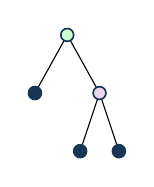
\begin{tikzpicture}[level distance=9mm,level 1/.style={sibling distance=10mm},level 2/.style={sibling distance=6mm},scale=.82,transform shape] \node[branch,fill=green!20] (n0) {} child {node[trueleaf] (n1) {}} child {node[branch,fill=violet!16] (n2) {} child {node[trueleaf] (n3) {}} child {node[trueleaf] (n4) {}}};\end{tikzpicture}\\[2pt]{\normalsize\texttt{\{1,\{1,1\}\}x147}}\end{minipage}\begin{minipage}[t]{.235\textwidth}\centering 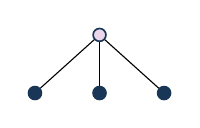
\begin{tikzpicture}[level distance=9mm,level 1/.style={sibling distance=10mm},level 2/.style={sibling distance=6mm},scale=.82,transform shape] \node[branch,fill=violet!16] (n0) {} child {node[trueleaf] (n1) {}} child {node[trueleaf] (n2) {}} child {node[trueleaf] (n3) {}};\end{tikzpicture}\\[2pt]{\normalsize\texttt{\{1,1,1\}x105}}\end{minipage}

{\footnotesize colored arity geometry; node color distinguishes constructors. Filled endpoints are true leaves; open endpoints are false/empty leaves. For colored grammars, color is genuine constructor data and is not silently converted into a positional zero pattern.}

{\footnotesize Typogeometric constructor codes and multiplicities: \(\Delta_{2}\!:\,7,\;\Delta_{3}\!:\,35,\;\Delta_{4}\!:\,105,\;\Delta_{5}\!:\,189,\;\Delta_{6}\!:\,189,\;\Delta_{7}\!:\,81\).}

\sectionbar{Coefficient and contour extraction}
{\footnotesize \[\begin{gathered}\mathcal K_n=\{(k_1,\ldots,k_6)\in\mathbb Z_{\ge0}^{6}:\sum_{j=1}^{6}jk_j=n-1\},\quad K=\sum_{j=1}^{6}k_j,\\a(n)=\frac{3}{n}\sum_{\boldsymbol k\in\mathcal K_n}\binom{n+K-1}{K}\binom{K}{k_1,\ldots,k_6}7^{k_1} 35^{k_2} 105^{k_3} 189^{k_4} 189^{k_5} 81^{k_6}.\end{gathered}\]}
\(a(n)=\dfrac{3}{2\pi i n}\oint_\gamma\dfrac{du}{\rho(u)^n},\quad n\ge1.\)

\sectionbar{Recurrence}
{\footnotesize \(\sum_{r=0}^{6}P_r(n)a(n+r)=0\) for \(n\ge 1\). The exact degree-6 coefficient polynomials are embedded in \texttt{certificate\_payload.json} (source: \texttt{release/certificate\_payload.json.gz\#/objects/p\_recurrence}).}

\sectionbar{Differential equation}
{\footnotesize The scalar linear ODE has order 6. It is obtained from the recurrence by the standard Euler-operator substitution. Exact coefficients and boundary polynomial: \texttt{release/certificate\_payload.json.gz\#/objects/ode\_from\_recurrence}.}

\sectionbar{Matrices, telescoper certificate, and checks}
{\small \(\text{No compact matrix tuple is shown; see the embedded exact reduction data.}\)}
\par\vspace{6pt}
{\small\textbf{Certificate.}\par\smallskip\(\displaystyle R(n,u)=N(n,u)/\rho(u)^{5},\ \deg_uN=36.\)\par}
\vspace{4pt}
{\small Telescoping identity: \(\sum_r P_r(n)H_{n+r}(u)=\partial_u\!\left(R(n,u)H_n(u)\right).\)\par}
\vspace{4pt}
{\footnotesize Matrix dimensions: \(14\times 14\); remainder \(6\times 7\), rank 6, nullity 1. The exact telescoping residual is zero. The recurrence reconstructs all 24 stored terms; 6/6 published OEIS prefix terms match.\par}

\vfill
\colorbox{soft}{\parbox{.97\textwidth}{\tiny Canonical records: \texttt{data/tree\_model.json}, \texttt{data/contour.json}, \texttt{data/matrices.json}, \texttt{data/recurrence.json}, \texttt{data/ode.json}. Embedded payload contains exact sources and SHA-256 matrix identifiers. Compare with the verbose certificate for A120590.}}
\end{document}
